\documentclass[a4wide]{report}

\usepackage{amsmath}
\usepackage[a4paper, total={7in, 10.2in}]{geometry}
\usepackage{graphicx}
\usepackage[portuguese]{babel}
\usepackage[utf8]{inputenc}


\begin{document}

\noindent
{\bf Rafael V. Cacilhas  - Relatório 02 (\today)}

\vspace{0.5cm}

\section*{Exercício 1}


\subsection*{1 a) }
Vamos calcular $f(x+h)$ e $f(x-h)$ expandindo a função $f(x)$ em série de Taylor:

\begin{equation}
\begin{cases}
f(x+h) = f(x) + h f'(x) + \frac{h^{2}}{2!}  f''(x) + O(h^{3})
 \\
f(x-h) = f(x) - h f'(x) + \frac{h^{2}}{2!}  f''(x) + O(h^{3}) 
 
 
 \end{cases}
\end{equation}

Subtraindo o segundo termo do primeiro, temos:

\begin{equation}
f(x+h) - f(x-h) = 2h f'(x)  +   O(h^{3})
\end{equation}

Isolando $f'(x)$, temos:

\begin{equation}
f'(x) =\frac{ f(x+h) - f(x-h)}{2h} -   O(h^{2})
\end{equation}

Note que o termo de ordem 3 passa a ser de ordem 2 visto que tudo foi dividido por h.


\subsection*{1 b) }
\begin{figure}[!htb]
\centering
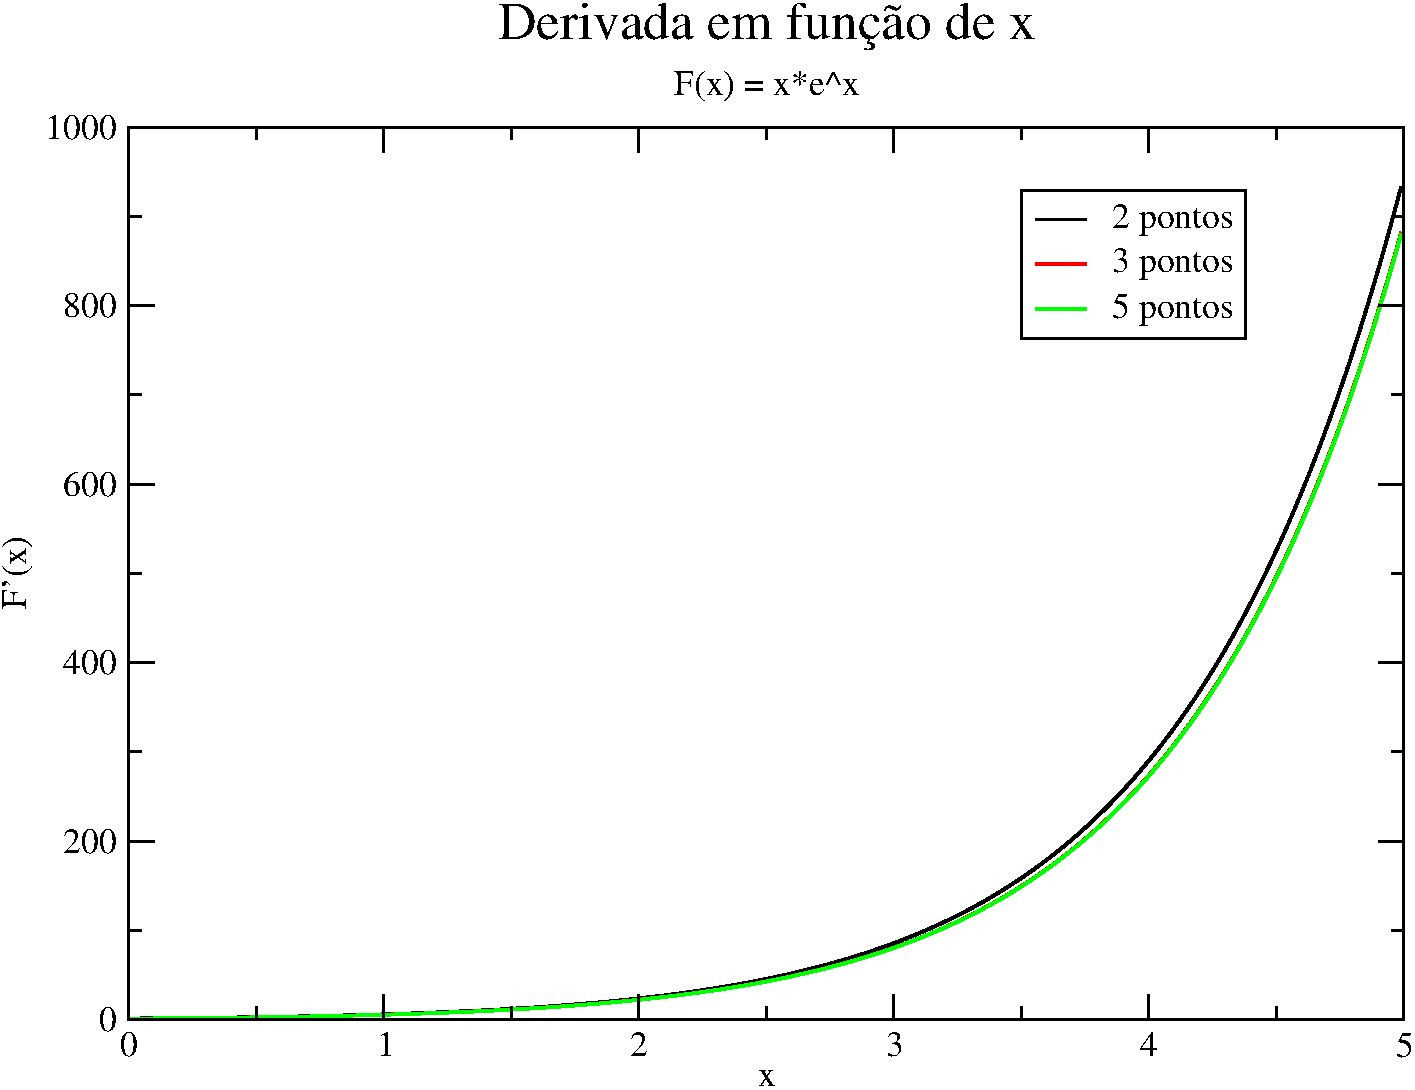
\includegraphics[width=0.447\textwidth]{derivadah1.pdf}
\caption{Derivadas da função para os três métodos diferentes para h = 0.10.}
\label{derivada}
\end{figure}

Na figura \ref{derivada}, onde h = 0.10, é possível ver que, na escala mostrada, os três métodos são bem parecidos para $x < 1$. Somente para $x > 3$ os métodos começam a apresentar alguma diferença, sendo que mesmo assim a diferença é apenas entre o método menos eficaz (2 pontos) e os outros dois. Fazer a variável h = 0.25 não muda o resultado significativamente e o gráfico portanto foi omitido.

\begin{figure}[!htb]
\centering
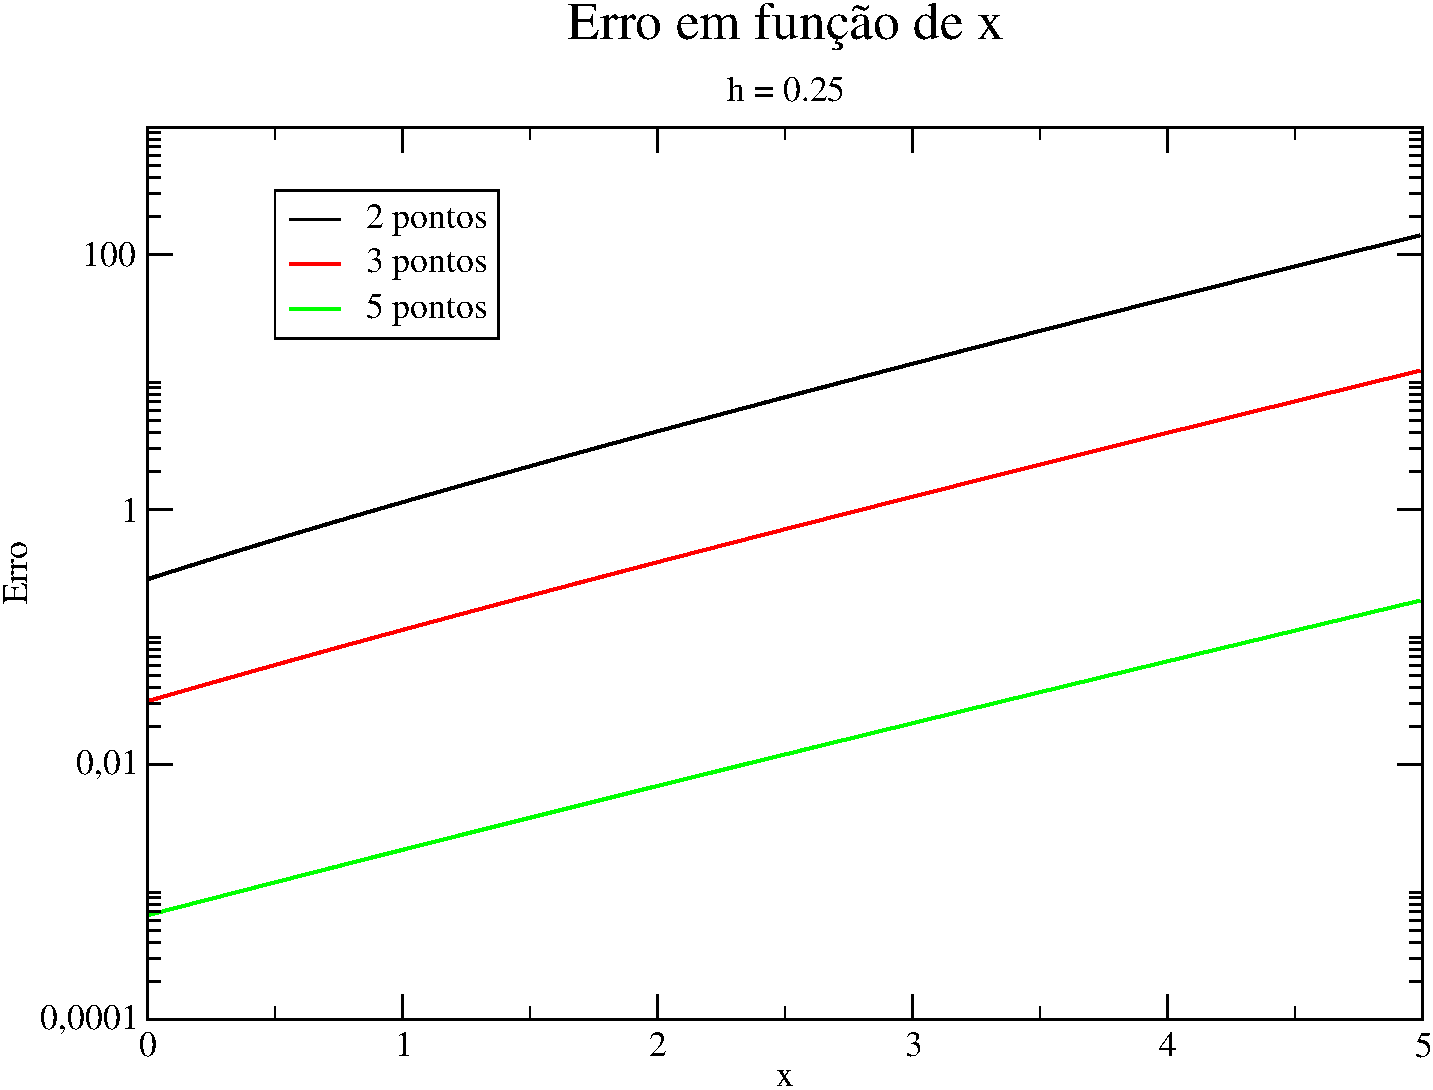
\includegraphics[width=0.447\textwidth]{erroh2log.pdf}
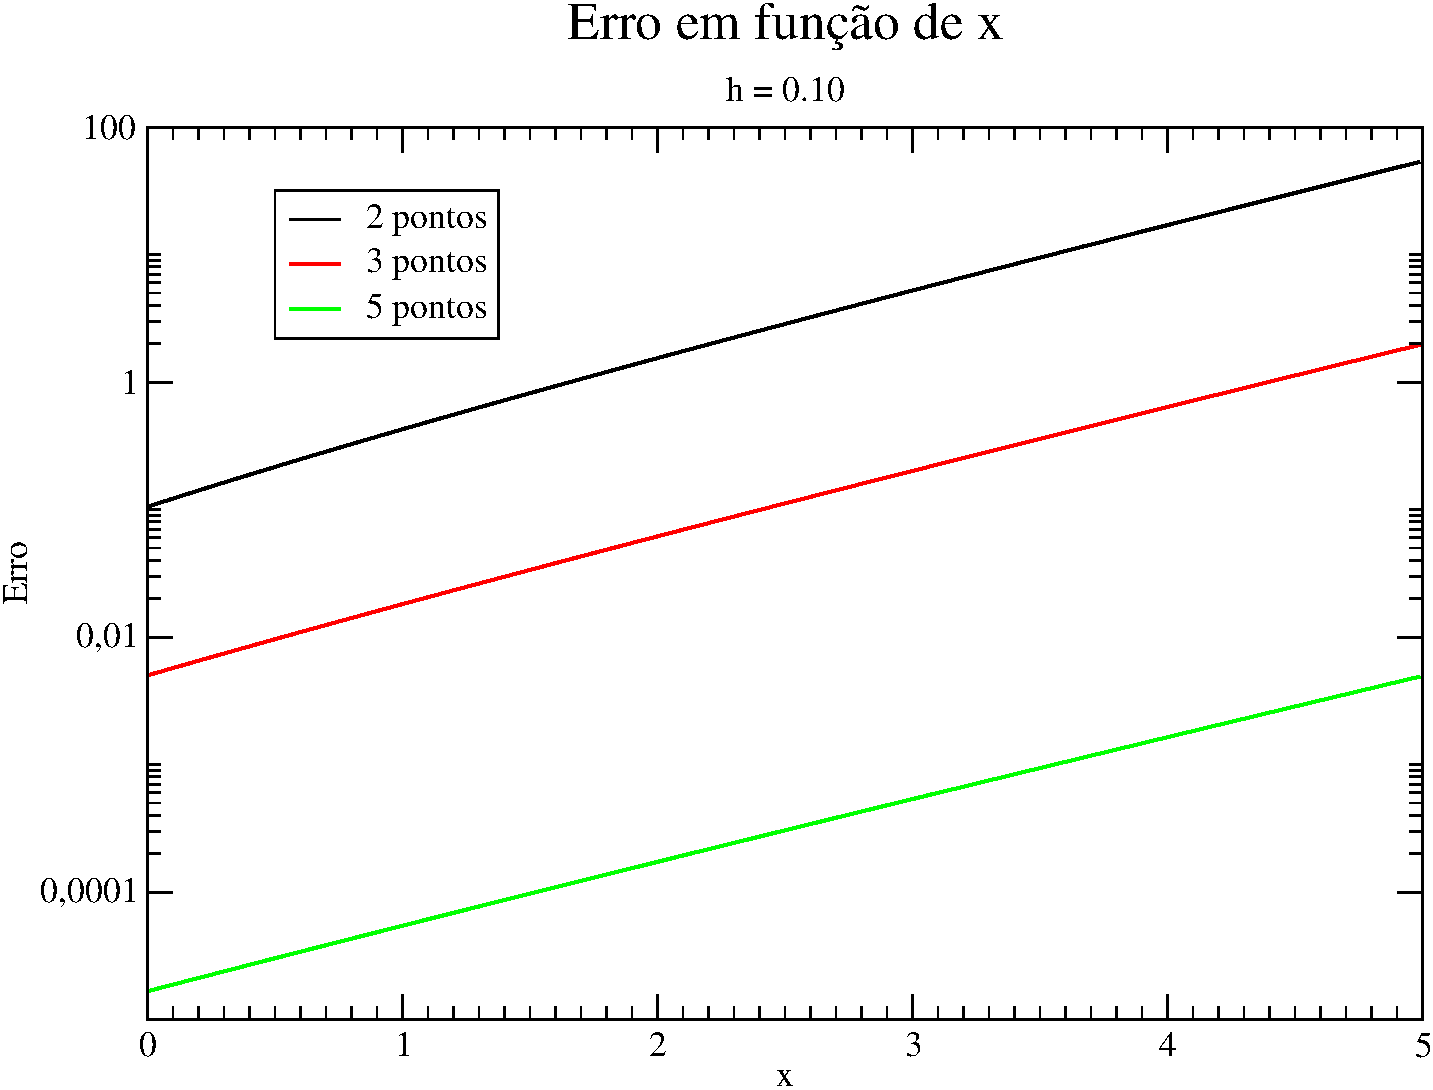
\includegraphics[width=0.45\textwidth]{erroh1log.pdf}%
\caption{Erro em função de x para h = 0.25(esquerda) e h=0.1(direita)}
\label{erro}
\end{figure}


O erro absoluto entre o valor numérico e o valor exato pode ser visto na figura \ref{erro}. Note que o erro associado a cada método é aproximadamente 3 vezes maior que o outro. A diferença entre h = 0.25 e h =0.10 faz com que o valor absoluto do erro caia em aproximadamente 2 vezes. 





\subsection*{1 c) }


O gráfico da segunda derivada através dos dois metodos pode ser visto na figura \ref{derivada2}. Nesta escala não é possivel determinar diferença alguma entre os dois métodos.

\begin{figure}[!htb]
\centering
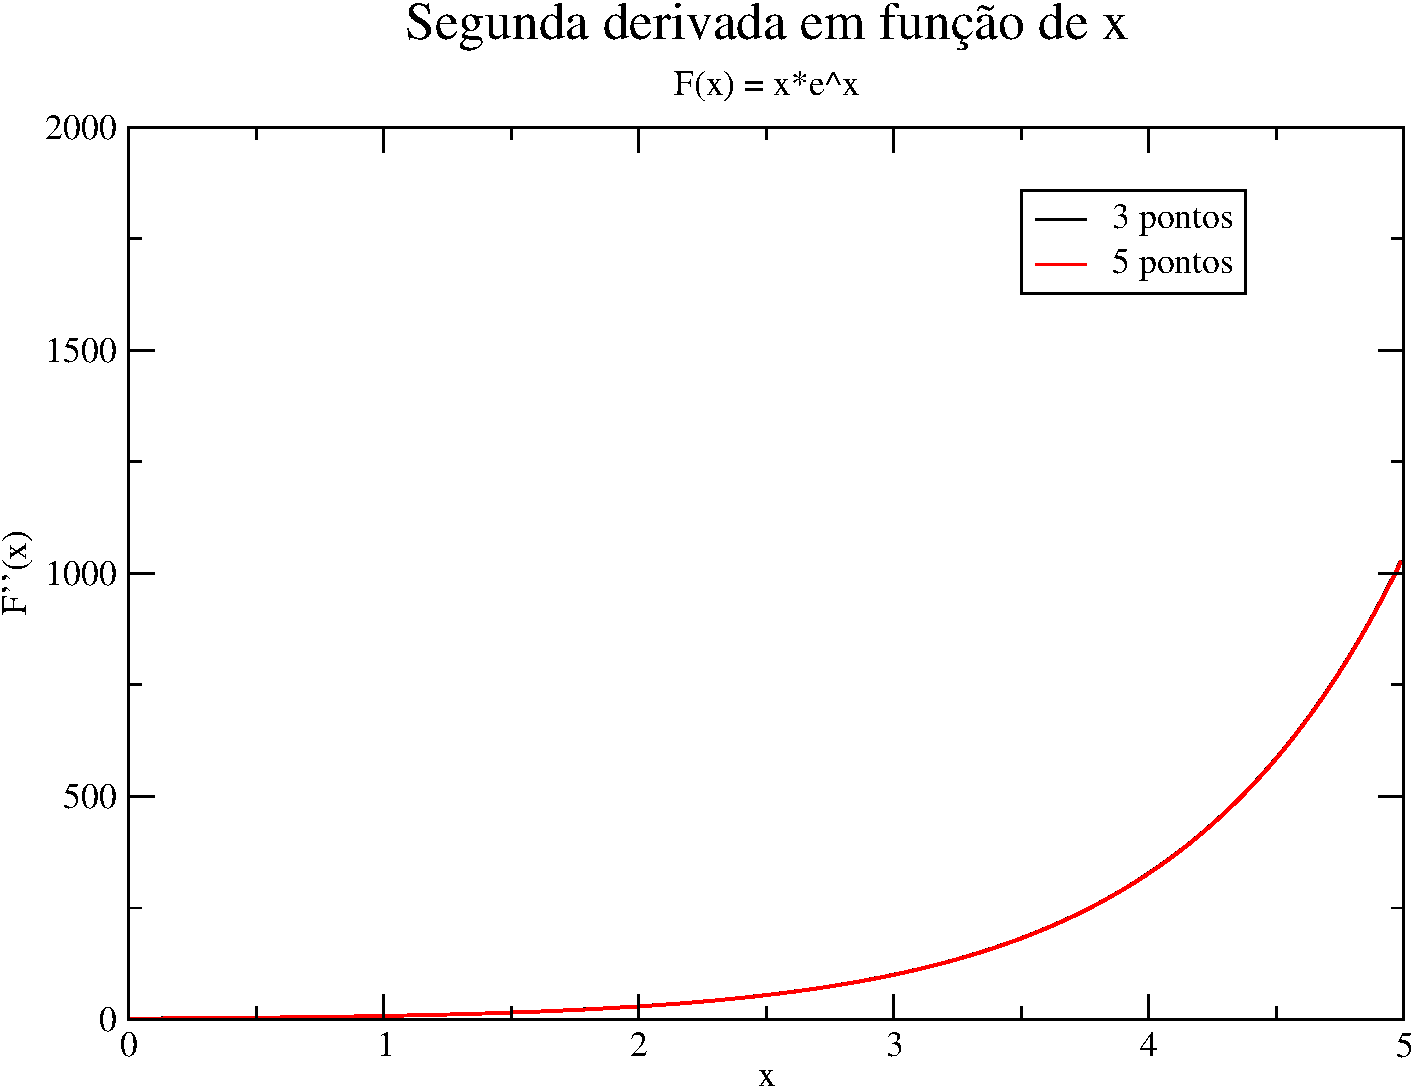
\includegraphics[width=0.447\textwidth]{derivada2h1.pdf}
\caption{Segunda derivada pelos dois métodos}
\label{derivada2}
\end{figure}


\begin{figure}[!htb]
\centering
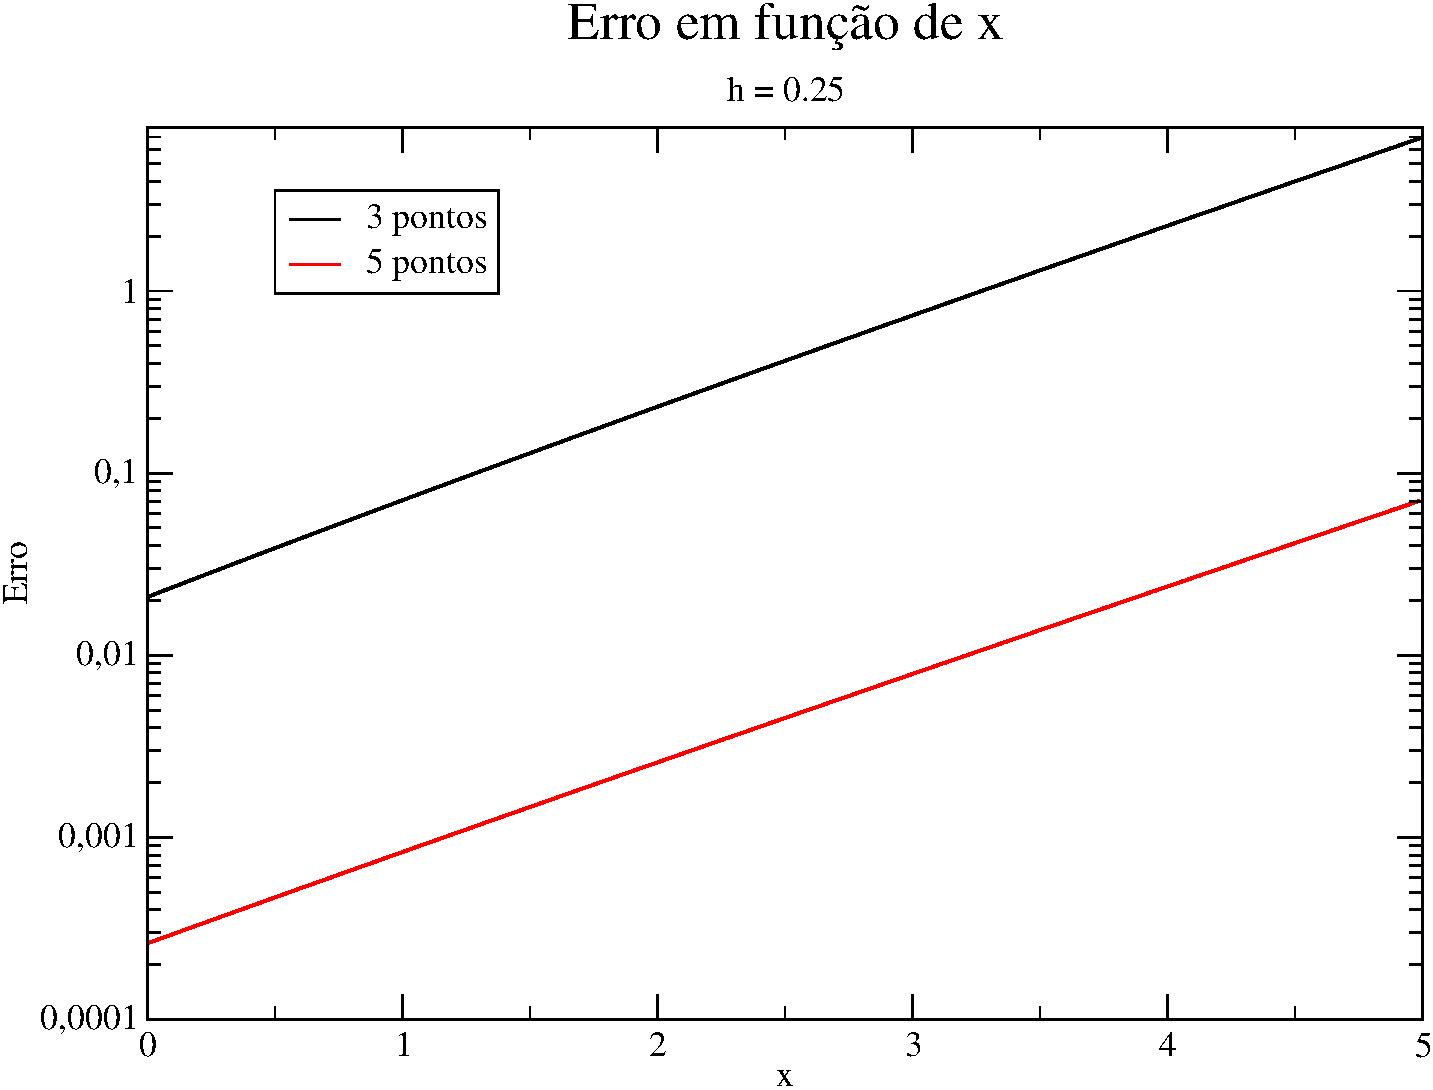
\includegraphics[width=0.45\textwidth]{erro2h2.pdf}%
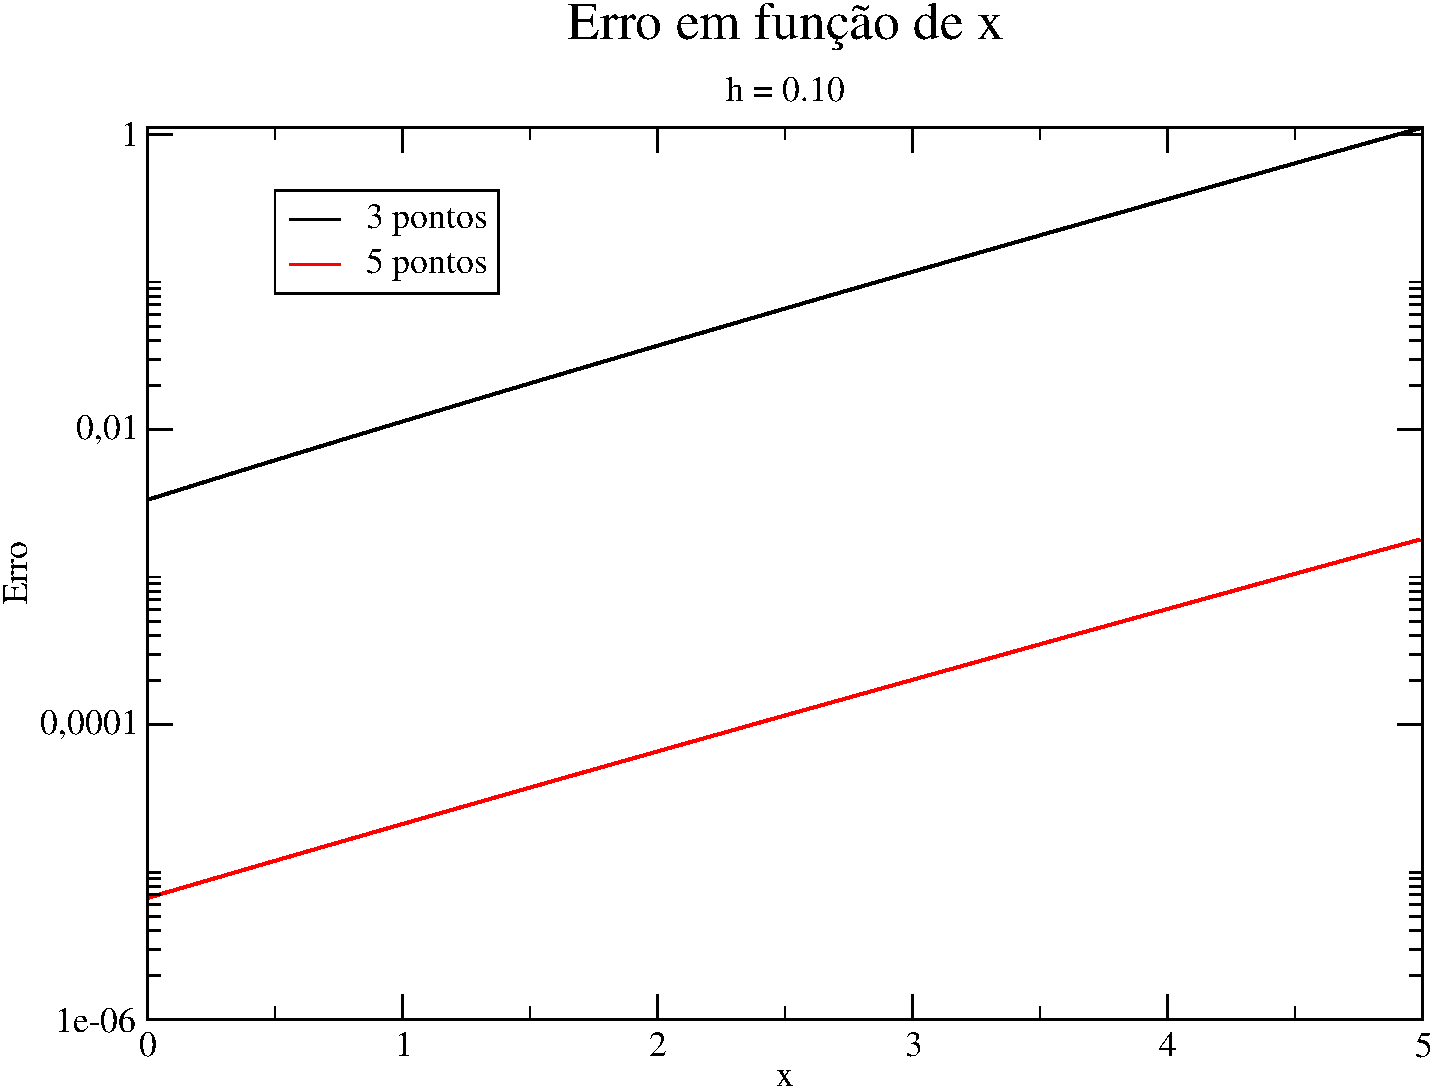
\includegraphics[width=0.447\textwidth]{erro2h1.pdf}
\caption{Erro da segunda derivada em função de x para h = 0.25(esquerda) e h=0.1(direita)}
\label{erro2}
\end{figure}

O erro absoluto, que pode ser visto na figura \ref{erro2}, foi de aproximadamente 10 vezes maior maior para o método menos efetivo. A mudança de h apresentou melhoras semelhantes à primeira derivada, apresentando erros aproximadamente 2 vezes menores.






\section*{Exercício 2}

\subsection*{a)}

\begin{figure}[!htb]
\centering
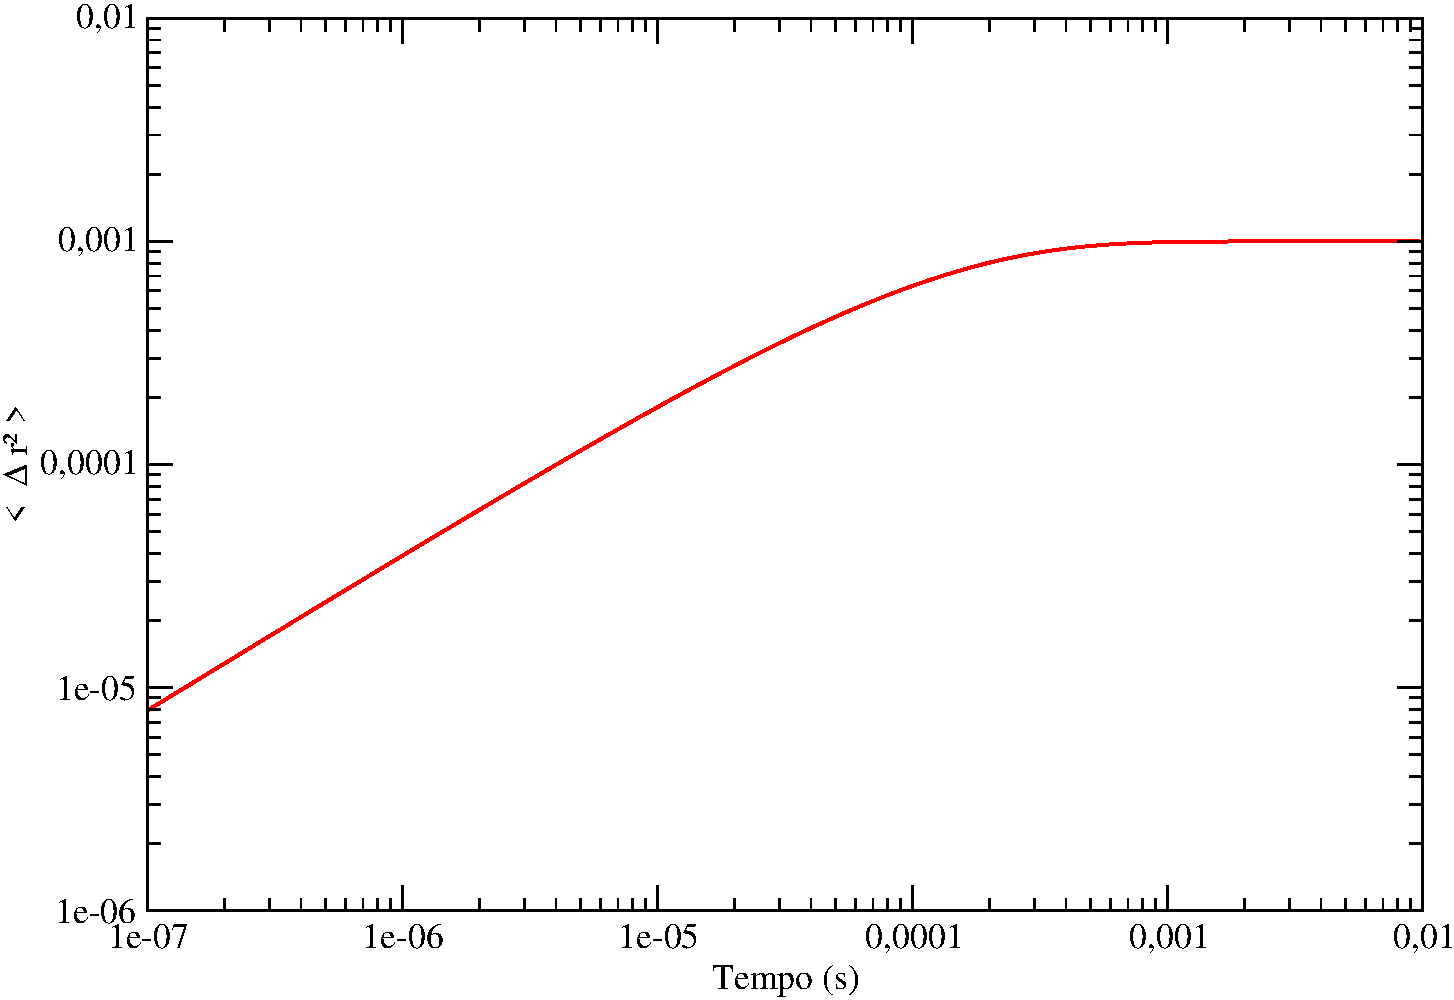
\includegraphics[width=0.447\textwidth]{deltar.pdf}
\caption{$<\Delta r^{2}>$ em função do tempo}
\label{deltar}
\end{figure}


Queremos que o intervalo entre $\log(x_{n})$ e $\log(x_{n+1})$ seja constante. Ou seja:


\begin{equation}
\log(x_{n+1}) - \log(x_{n}) = k
\end{equation}

Com uma simples álgebra chegamos que:

\begin{equation}
x_{n+1} = x_{n}\times 10^{k}  = C x_{n} 
\end{equation}

Por indução finita, temos:


\begin{array} 
{lcl} x_{1} = C x_{0}  \\  x_{2} = C^{2} x_{1}   \\ ... \\ x_{n} = C^{n} x_{0} 
\end{array}

Como controlamos o valor inicial de x e o número N de pontos que temos, chegamos em:
\begin{equation}
C = \left( \frac{x_{N}}{x_{0}} \right)^{1/N}  
\end{equation}




\subsection*{b)}
Note que:

\begin{equation}
\beta (t) = \frac{\partial \ln(f(t))}{\partial \ln(t)} =   \frac{\partial \ln(f(t))}{\partial t} \frac{\partial t}{\partial \ln(t)}  = \frac{1}{f}\frac{\partial f(t)}{\partial t}t
\end{equation}

A analise da figura $\ref{beta}$ mostra que o valor de $\beta$ permanece aproximadamente constante até tempos da ordem de $2\times10^{-6}$s, assumindo um valor aproximado de 0.7.
\begin{figure}[!htb]
\centering
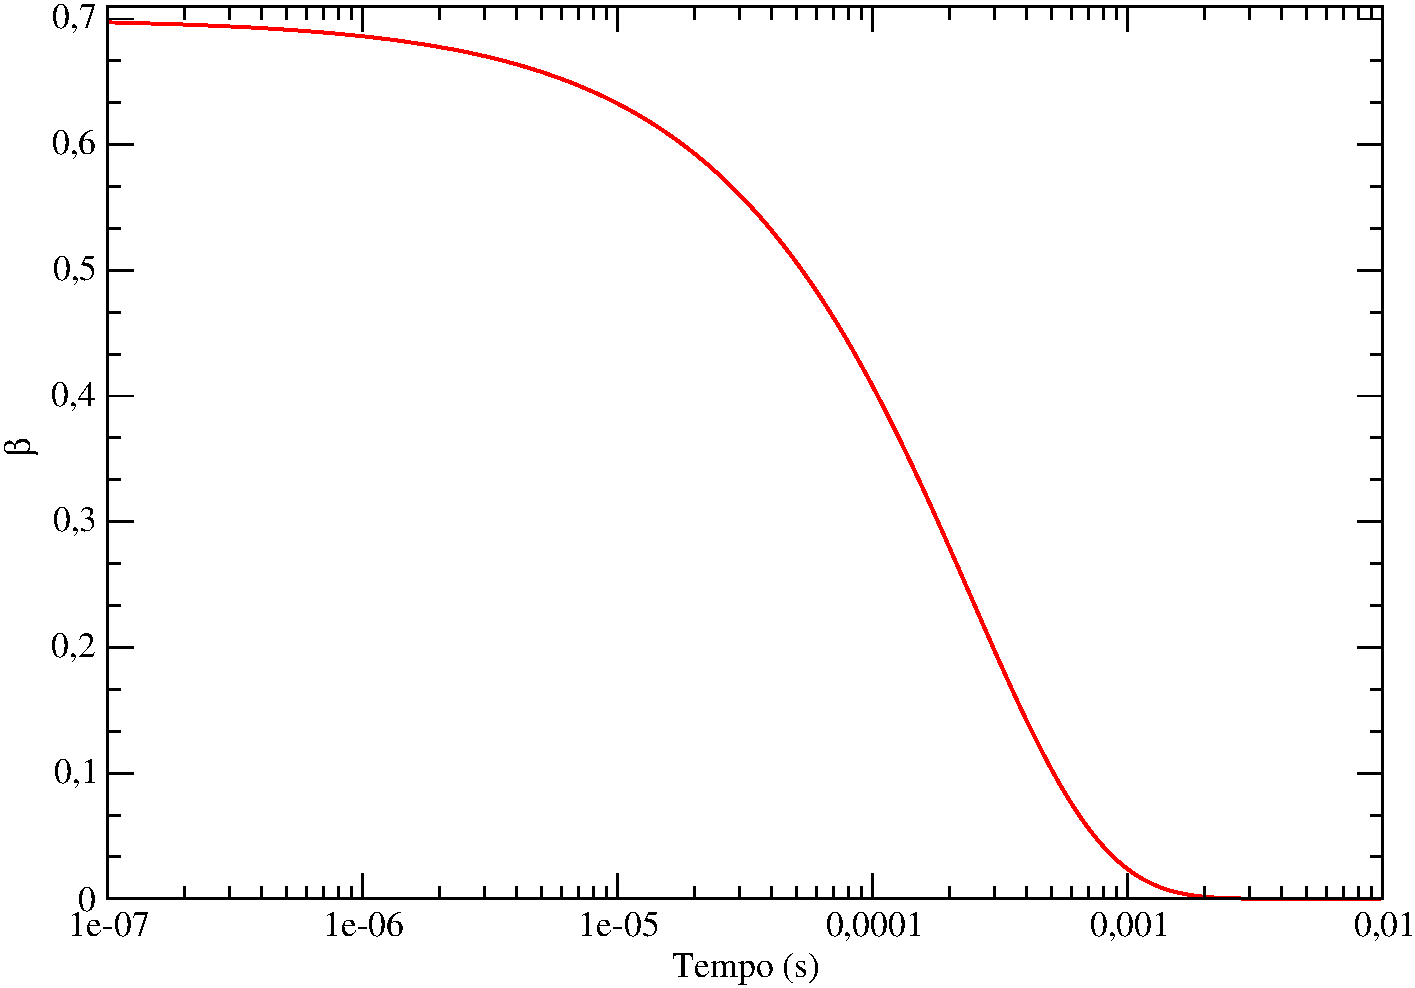
\includegraphics[width=0.447\textwidth]{beta2log.pdf}
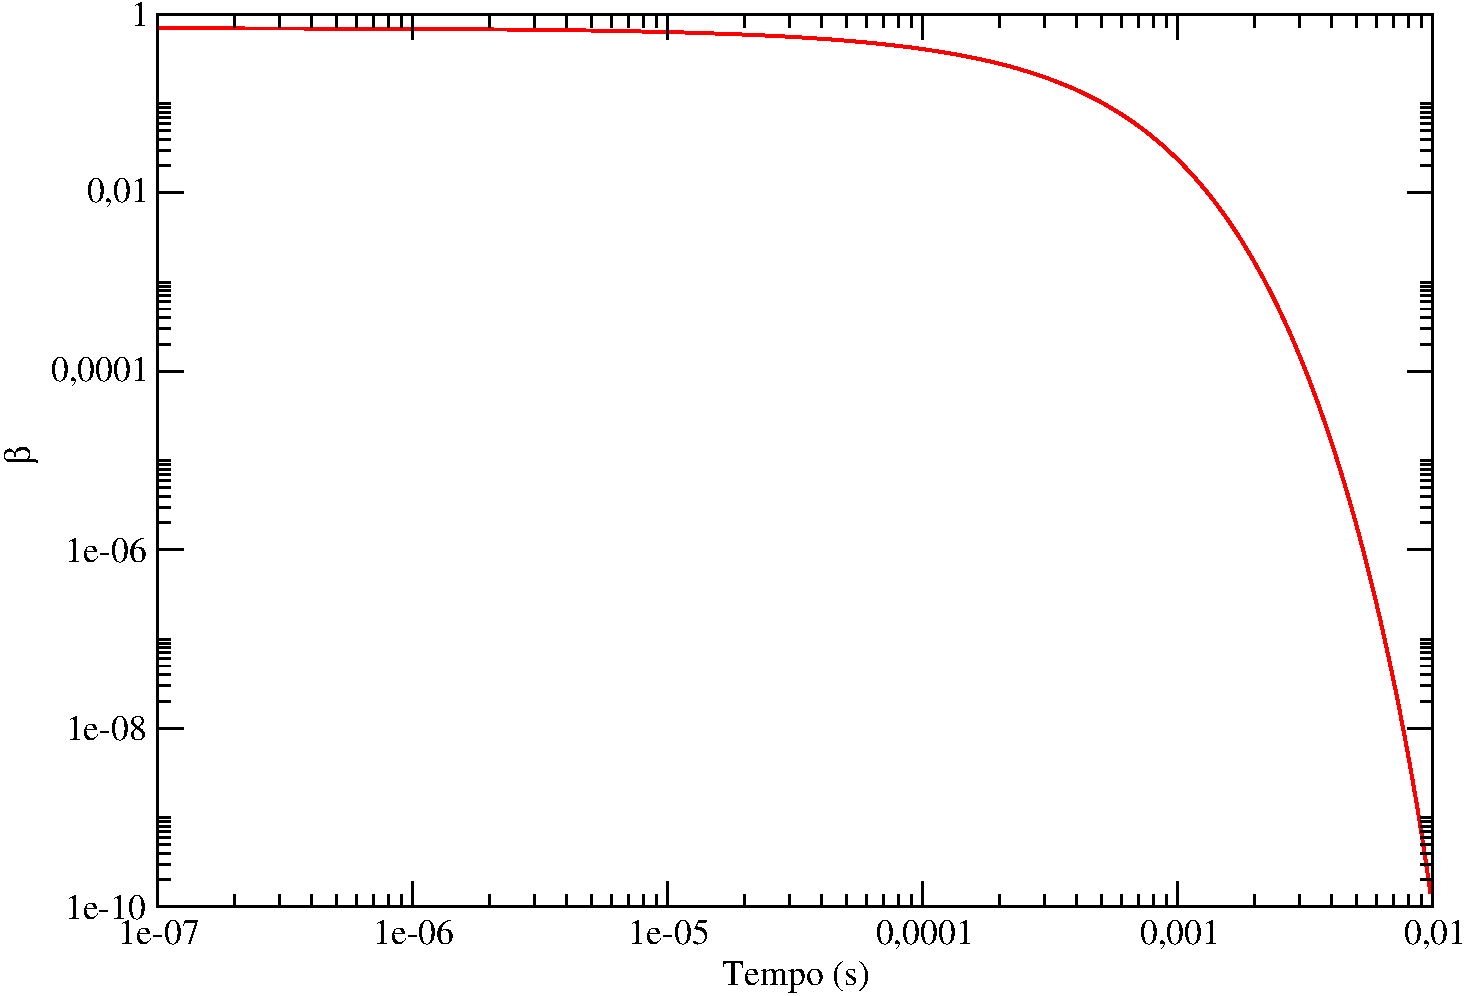
\includegraphics[width=0.447\textwidth]{beta2.pdf}
\caption{ $\beta$  em função do tempo, em escala linear-log e log-log}
\label{beta}
\end{figure}

Como os pontos no eixo x foram feitos para serem igualmente espaçados em escala log-log não há problema em derivar os logaritmos perto dos pontos iniciais e finais, visto que ainda estão igualmente espaçados.




\section*{Exercício 3}
\subsection*{a)}
Neste método a raíz obtida depende exclusivamente do valor do "chute" $x_{0}$. Assim, se torna necessário escolher diversos $x_{0}$ de modo a garantir que todas as raízes no intervalo foram encontradas. Foi escolhido começar em $x_{0} = -2.0 $ e aumentar $x_{0}$ em uma unidade por 80 vezes. Escolhemos mostrar como resultado o primeiro $x_{0}$ que convergiu para cada raíz, ao invés do $x_{0}$ mais próximo ou de convergência mais rápida. 

Para evitar que a mesma raíz seja descoberta várias vezes foi feito um algoritmo no programa para eliminar raízes repetidas.Também foi feito um algoritmo para eliminar raízes fora do intervalo de interesse. As raízes encontradas estão na tabela 1.

\begin{table}[]
\centering

\begin{tabular}{lllll}
\hline
Raíz                & Erro                    & $X_{0}$ & Nº de iterações &  \\
\hline
-31.420985840138805 & $1.04\times 10^{-6}$ &  6         & 5               &  \\
\hline
-15.687728886072014 & $1.27\times 10^{-8}$ &  5         & 10              &  \\
\hline
-1.5258623165372684 & $1.04\times 10^{-6}$ & -2         & 4               &  \\
\hline
 15.728094338345299 & $5.94\times 10^{-5}$ & 10         & 5               &  \\
 \hline
 31.410863973802925 & $1.58\times 10^{-6}$ & 0          & 6               & 
\end{tabular}
\label{tabela3}
\caption{Solução do exercício 3.}
\end{table}

Como podemos ver há pouquissima correlação entre a raíz encontrada e o chute inicial. Certamente existem valores de $x_{0}$ mais próximos à raiz que trarão uma convergência mais rápida, mas como o método é extremamente rápido e portanto não foi necessário otimiza-lo para este fim.

\subsection*{b)}

Os resultados estão na figura \ref{iteracao}. O número de iterações variou entre 3 e 6, o que demonstra a rápida convergencia do método e o motivo pelo qual se escolheu repetir os métodos para tantos $x_{0}$. diferentes
\begin{figure}[h]
\centering
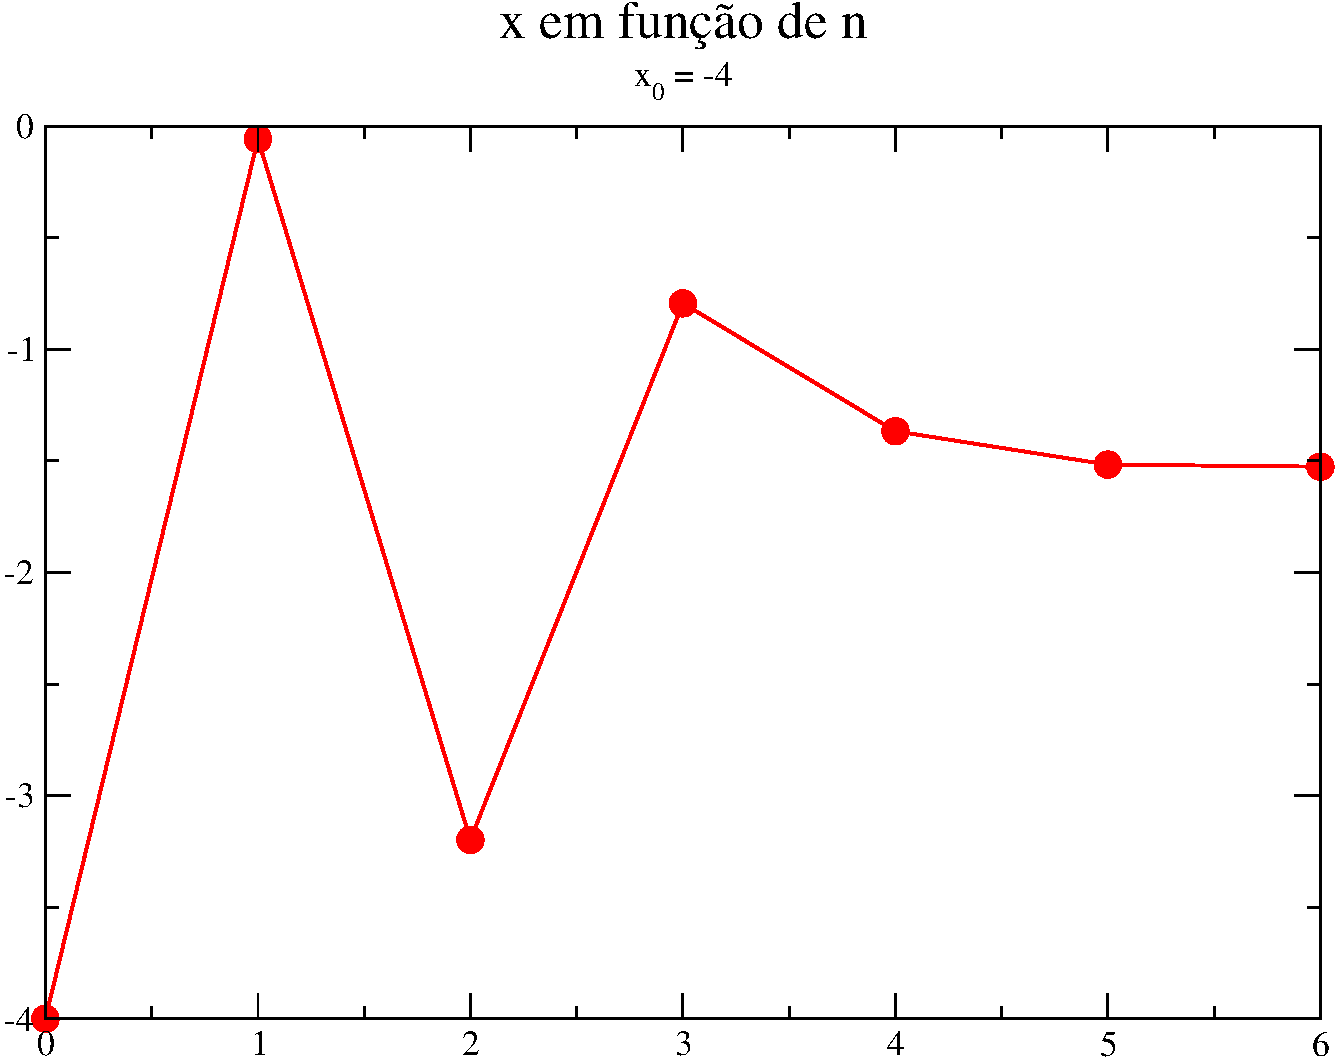
\includegraphics[width=0.447\textwidth]{4.pdf}
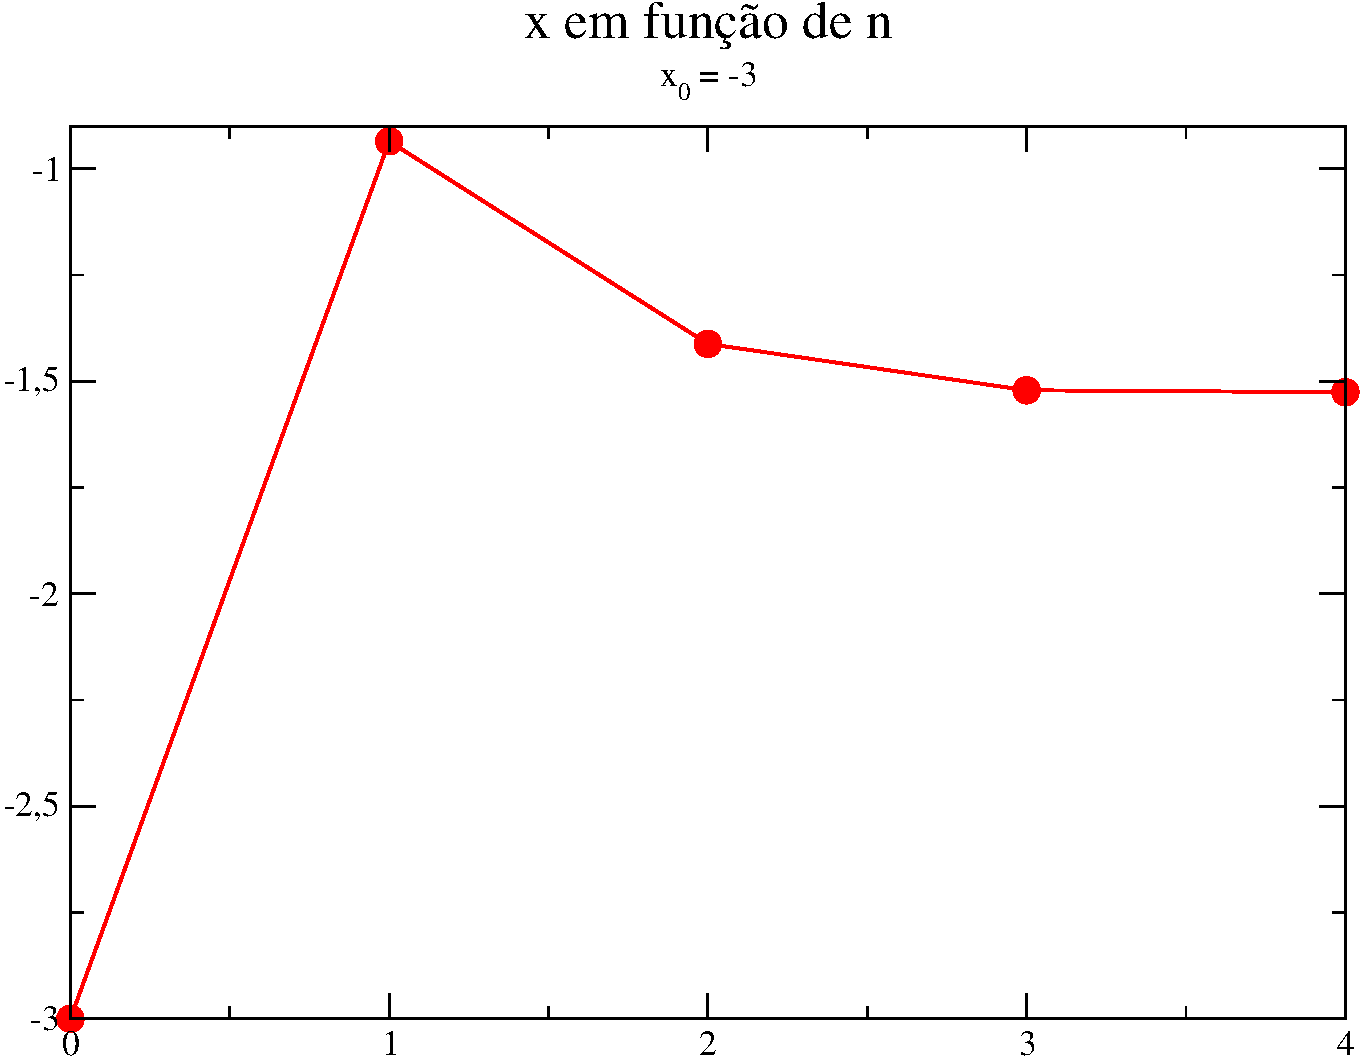
\includegraphics[width=0.447\textwidth]{3.pdf}
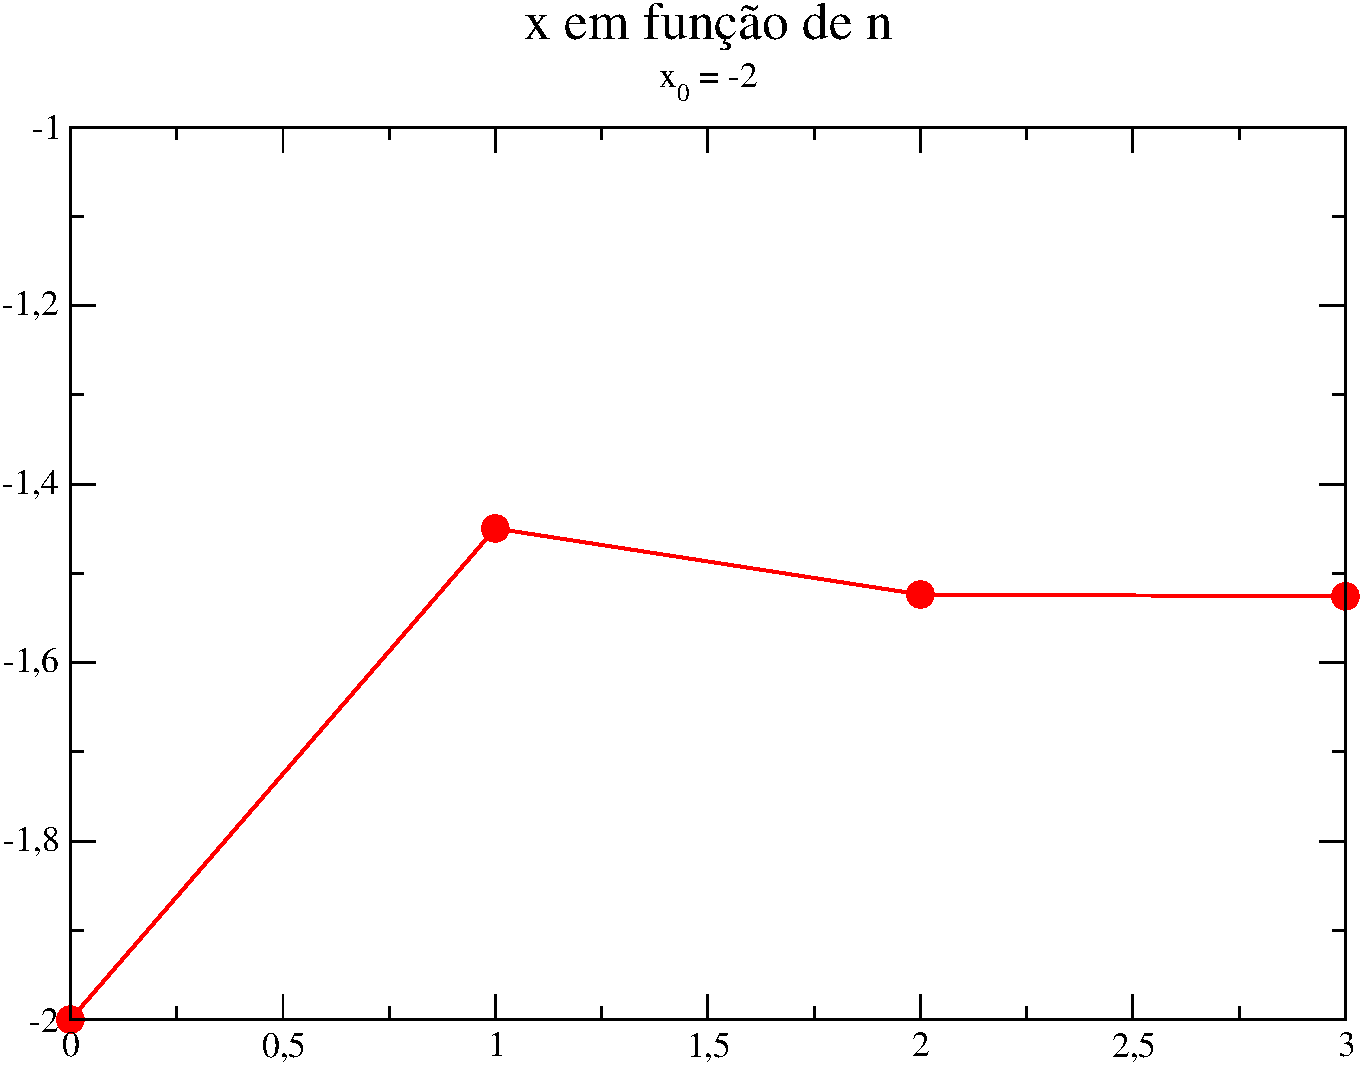
\includegraphics[width=0.447\textwidth]{2.pdf}
\caption{Valor de x para cada iteração para três valores de $x_{0}$.}
\label{iteracao}
\end{figure}




\section*{Exercício 4}
\subsection*{a)}
Vamos escrever f(x) através da sua série de Taylor centrada em algum ponto i:

\begin{equation*}
f(x-i) = f(i) + (x-i) f'(i) +   O(h^{2})

\label{int1}
\end{equation}



Mas podemos escrever a derivada como:

\begin{equation*}
f'(i)  =  \frac{f(i+1)-f(i	)}{h} +   O(h)

\label{int1}
\end{equation}
	
Onde usamos a derivada de dois pontos, o que introduz um erro da ordem de h.

\begin{equation*}
f(x-i)  = f(h) + (x-i) \left(\frac{f(i+1)-f(i	)}{h} +   O(h) \right) +   O(h^{2})

\label{int1}
\end{equation}

Integrando de x = i ate i+1:
\begin{equation*}
\int_{i}^{i+1} f(x) dx   =\int_{2i}^{2i+1} f(i) + (x-i) \left(\frac{f(i+1)-f(i	)}{h} +   O(h) \right) +   O(h^{2}) dx

\end{equation}

Fazendo x-i = u:
\begin{equation*}
\int_{i}^{i+1} f(x) dx = u f(i) + \frac{u^{2}}{2} \left(\frac{f(i+1)-f(i	)}{h} +   O(h) \right) +   O(h^{3}) 
\end{equation}


\begin{equation*}
\int_{i}^{i+1} f(x) dx = h f(h) + \frac{h^{2}}{2} \left(\frac{f(i+1)-f(i	)}{h} +   O(h) \right) +   O(h^{3}) 
\end{equation}
\begin{equation*}
\int_{i}^{i+1} f(x) dx =  \frac{f(i+1)+f(i	)}{2h}    +   O(h^{3}) 
\end{equation}
Ou seja, a aproximação é válida para ordem de $h^{3}$.

\subsection*{b)}
 Os resultados estão apresentados na tabela 2.
\begin{table}[]
\centering
\label{table:tabela4}
\begin{tabular}{lllll}
\hline
         & N = 100             & Erro_{100}            & N = 1000            & Erro_{1000}           \\
         \hline
Trapézio & 0.99997948194895436 & -2.0518051045637087$\times 10^{-5}$ & 0.99999983809459891 & -1.6190540108595997$\times 10^{-7}$ \\
\hline
Simpsons & 1.0000000437325294  & 4.3732529375617446$\times 10^{-8}$  & 1.0000000437113910  & 4.3711390951273188$\times 10^{-8}$  \\
\hline
         &                     &                          &                     &                         
\end{tabular}

\caption{Solução do exercício 4.}
\end{table}

Note que os erros do trapézio estão coerentes com a teoria: para N = $10^{2}$  temos um erro perto de $10^{-4}$  e para N = $10^{3}$ temos um erro proximo a $10^{-6}$. O método de Simmons, no entando, apresenta um erro coerente somente para N = $10^{2}$, onde o erro é da ordem de $10^{-8}$. Para N = $10^{3}$, onde seria esperado um erro de $10^{-12}$ ainda obtemos um erro da ordem de $10^{-8}$. Isto provavelmente se deve ao fato de utilizarmos variaveis reais*8 e estarmos perto do limite de precisão.    

\section*{Exercicio 5}

\subsection*{a)}
Um esboço inicial da funçao g mostra que ela assume valores aceitaveis quando a energia é da ordem de $10^{-22}$, sendo que g assume valores da ordem de $10^{47}$. Fora deste intervalo a função é praticamente nula em todos os pontos.

Para trabalhar em dimensões razoaveis, iremos utilizar a energia em micro eletron-volts, o que faz com que o eixo x diminua por um fator de $10^{-25}$ e o eixo y por um fator de $10^{-12}$ . Poderíamos também trabalhar com o número de mol ao invés do número de moléculas, o que faria g cair mais 22 ordens de grandeza. No entanto estamos atrás de N, que tem ordem de grandeza de $10^{13}$, e fazer que ele caia 22 ordens de grandeza não irá ajudar de maneira significativa. Não iremos utilizar essa opção, mas é interessante saber que ela exista caso outro exemplo utilize um número maior de N. 



A integral imprópria é facilmente calculada analíticamente e nos mostra que o valor exato do número de partículas é $N = 1.5 \times 10^{13}$.

\begin{figure}[!b]
\centering
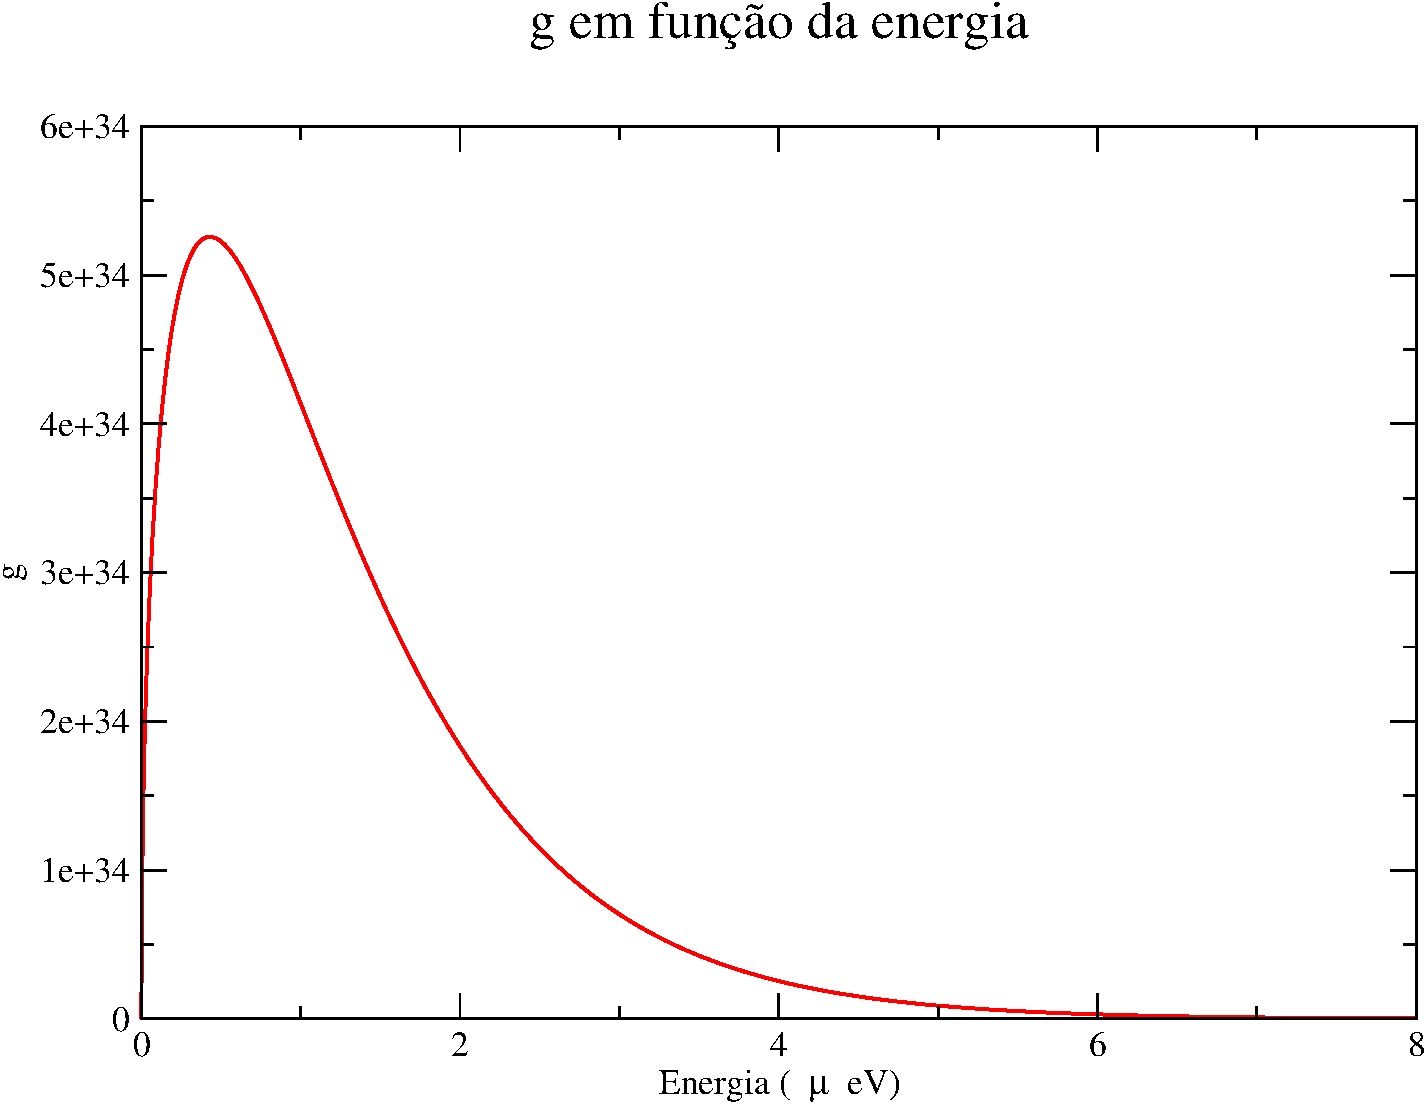
\includegraphics[width=0.447\textwidth]{g.pdf}
\caption{Densidade de particulas em função da energia}
\label{g}
\end{figure}



\subsection*{b)}

Na tabela 3 apresentamos o N encontrado para três valores de a. Como pode-se observar, estamos bem proximo do valor esperado $N = 1.5 \times 10^{13}$.
\begin{table}[]
\centering
\begin{tabular}{lllll}
\hline
  & a =10               & a = 25                    & a = 50              &  \\
  \hline
N &  $1.535\times10^{13}$   &  $1.509\times10^{13}$ &    $1.503\times10^{13}$   &  \\
\hline

\end{tabular}
\label{tabela5}
\caption{Solução do exercício 5.}
\end{table}


\end{document}
